\documentclass[12pt,letterpaper]{article}
\usepackage[spanish,es-nodecimaldot]{babel}
\usepackage[utf8]{inputenc}
\usepackage[T1]{fontenc}
\usepackage{geometry}
\usepackage{graphicx}
\usepackage{booktabs}
\usepackage{amsmath,amssymb}
\usepackage{float}
\usepackage{caption}
\usepackage{subcaption}
\usepackage{longtable}
\geometry{margin=2.5cm}
\graphicspath{{figuras/}}

\title{Modelo multivariado de machine learning para la predicción y simulación del precio del oro}
\author{Alejandro Ramirez \and Leidy Paola Patiño}
\date{\today}

\begin{document}
\maketitle

\begin{abstract}
Este trabajo desarrolla un modelo multivariado para predecir el precio del oro a partir de información histórica del XAU/USD, precios de la plata, precios utilizados en reportes NI 43-101 y variables macroeconómicas disponibles. Inicialmente se había seleccionado XGBoost por presentar el menor error promedio en validación temporal frente a otros modelos. En esta versión mejorada se amplió la comparación a LightGBM, CatBoost, Random Forest, Extra Trees, HistGradientBoosting y una búsqueda automática con Optuna. El objetivo supervisado fue el log-retorno del precio de cierre del oro al siguiente día hábil, evitando fuga de información. El modelo seleccionado por menor RMSE promedio en validación temporal fue LightGBM optimizado por Optuna, mientras que CatBoost presentó el menor RMSE en la ventana final de prueba. Finalmente, se construyeron escenarios de pronóstico y simulaciones Monte Carlo hasta 2035.
\end{abstract}

\textbf{Palabras clave:} oro, machine learning, XGBoost, LightGBM, CatBoost, Monte Carlo, NI 43-101, series de tiempo.

\section{Introducción}
El precio del oro es una variable relevante para la evaluación económica de proyectos mineros, la estimación de recursos y reservas, la planeación financiera y el análisis de riesgo. Su comportamiento depende de factores financieros, macroeconómicos y de mercado, entre ellos tasas de interés, inflación, dólar, volatilidad, precios de metales relacionados y expectativas de inversión.

El trabajo parte de una base histórica del precio del oro entre 2016 y 2026. En una etapa inicial se compararon varias configuraciones de modelos y se seleccionó XGBoost porque obtuvo el menor error en validación temporal. En la versión mejorada se conservó esa lógica metodológica, pero se amplió el conjunto de modelos y se integró optimización automática de hiperparámetros con Optuna.

\subsection{Objetivo general}
Construir, validar y documentar un modelo multivariado de machine learning para estimar el comportamiento del precio del oro y generar escenarios de simulación hasta 2035, con énfasis en la comparación de modelos, la selección por error temporal y la interpretación de resultados mediante gráficas y métricas.

\subsection{Objetivos específicos}
\begin{itemize}
    \item Consolidar una base de datos con precio histórico del oro, precio de la plata, precios NI 43-101 y variables macroeconómicas disponibles.
    \item Construir variables explicativas de tipo técnico, temporal, macroeconómico y minero.
    \item Comparar modelos de machine learning bajo validación temporal, evitando fuga de información.
    \item Seleccionar el modelo con menor RMSE promedio en validación temporal.
    \item Generar pronósticos de corto plazo para mayo, junio y julio de 2026.
    \item Construir escenarios de largo plazo hasta 2035 mediante simulación Monte Carlo.
    \item Presentar resultados en reportes, gráficas, archivos editables y un tablero de visualización.
\end{itemize}

\subsection{Alcance del trabajo}
El modelo no pretende entregar un precio exacto e invariable del oro. Su objetivo es producir un pronóstico condicional a la información disponible y una distribución de escenarios posibles. Por esta razón, los resultados de largo plazo se interpretan como simulaciones con incertidumbre, no como valores determinísticos. El análisis es útil para sensibilidad, discusión económica y apoyo a decisiones, pero no reemplaza una valoración financiera completa ni una evaluación de riesgos de mercado profesional.

\section{Marco teórico}
\subsection{Predicción de series financieras}
Las series financieras suelen presentar ruido, cambios de tendencia, volatilidad variable y dependencia temporal. Por ello, en lugar de predecir directamente el nivel del precio, se modeló el log-retorno de un día adelante:
\begin{equation}
r_{t+1}=\ln\left(\frac{P_{t+1}}{P_t}\right),
\end{equation}
donde $P_t$ es el precio de cierre del oro en el día $t$. Luego, el precio predicho se reconstruye como:
\begin{equation}
\hat{P}_{t+1}=P_t e^{\hat{r}_{t+1}}.
\end{equation}

\subsection{Variables técnicas}
Se construyeron rezagos, diferencias, retornos, medias móviles y volatilidades. Una media móvil simple de ventana $k$ se calcula como:
\begin{equation}
MA_k(t)=\frac{1}{k}\sum_{i=0}^{k-1}P_{t-i}.
\end{equation}
La volatilidad móvil se estimó como la desviación estándar de los retornos recientes:
\begin{equation}
\sigma_k(t)=\sqrt{\frac{1}{k-1}\sum_{i=0}^{k-1}\left(r_{t-i}-\bar{r}_k\right)^2}.
\end{equation}

\subsection{Modelos evaluados}
Se evaluaron modelos de árboles y boosting. XGBoost y LightGBM son métodos de gradient boosting que construyen ensambles de árboles secuenciales. CatBoost es otro modelo de boosting robusto para relaciones no lineales. Random Forest y Extra Trees son ensambles basados en múltiples árboles entrenados con aleatoriedad. HistGradientBoosting es una implementación eficiente de boosting por histogramas.

\subsection{LightGBM y Optuna}
LightGBM fue el modelo seleccionado en la versión mejorada. Es un método de gradient boosting basado en árboles que construye muchos árboles secuenciales. Cada árbol busca corregir errores residuales de los árboles anteriores. La predicción final puede entenderse como una suma ponderada de árboles:
\begin{equation}
\hat{r}_{t+1}=F_0(X_t)+\eta\sum_{m=1}^{M}f_m(X_t),
\end{equation}
donde $X_t$ es el conjunto de variables explicativas, $f_m$ es el árbol $m$, $M$ es el número de árboles y $\eta$ es la tasa de aprendizaje.

Optuna se utilizó para buscar automáticamente hiperparámetros. En lugar de elegir manualmente todas las configuraciones, Optuna propuso combinaciones de parámetros, entrenó modelos y seleccionó la configuración que redujo el RMSE promedio de validación temporal. El objetivo de la optimización fue:
\begin{equation}
\min_{\theta} RMSE_{CV}(\theta),
\end{equation}
donde $\theta$ representa los hiperparámetros de LightGBM.

\section{Materiales y métodos}
\subsection{Datos}
El archivo base fue \texttt{historicoauplata.xlsx}. Se usaron las hojas \texttt{historicos}, \texttt{plata} y \texttt{ni}. También se consultaron series macroeconómicas externas desde FRED cuando estuvieron disponibles. La base final de modelado incluyó 76 variables explicativas después de limpieza y construcción de características.

\begin{table}[H]
\centering
\caption{Fuentes de información utilizadas.}
\begin{tabular}{lp{9cm}}
\toprule
Fuente & Uso dentro del modelo \\
\midrule
Históricos del oro XAU/USD & Serie principal de precio de cierre, variable objetivo y variables técnicas. \\
Precio de la plata & Variable exógena para capturar relación entre metales preciosos. \\
Reportes NI 43-101 & Precios de recursos y reservas usados como referencia minera. \\
FRED & Variables macroeconómicas disponibles, como CPI, fed funds y S\&P 500. \\
Calendario & Año, mes, trimestre, día de semana y ciclos senoidales. \\
\bottomrule
\end{tabular}
\end{table}

\subsection{Flujo metodológico}
El flujo de trabajo aplicado fue:
\begin{enumerate}
    \item Lectura automática del archivo de datos.
    \item Detección de la hoja histórica del oro y de la columna objetivo.
    \item Limpieza de fechas, precios y valores faltantes.
    \item Integración de plata, NI 43-101 y variables macroeconómicas.
    \item Construcción de variables explicativas.
    \item Definición del objetivo como log-retorno de un día adelante.
    \item Separación temporal en entrenamiento y prueba.
    \item Validación temporal con varios modelos.
    \item Selección del modelo por menor RMSE promedio de validación.
    \item Pronóstico recursivo y simulación Monte Carlo por escenarios.
    \item Generación de reportes, gráficas, archivos CSV/Excel y tablero.
\end{enumerate}

\subsection{Variables explicativas}
Las 76 variables se organizaron en grupos. La Tabla \ref{tab:variables_grupo} resume la lógica de cada grupo.

\begin{table}[H]
\centering
\caption{Grupos de variables explicativas.}
\label{tab:variables_grupo}
\begin{tabular}{lp{9cm}}
\toprule
Grupo & Ejemplos e interpretación \\
\midrule
Nivel de precios & \texttt{precio\_oro}, \texttt{precio\_plata}. Representan el estado actual del mercado. \\
Rezagos & \texttt{precio\_oro\_lag\_1}, \texttt{precio\_oro\_lag\_20}. Capturan memoria temporal. \\
Retornos y diferencias & \texttt{retorno\_oro\_5}, \texttt{diferencia\_oro\_10}. Capturan cambios recientes. \\
Medias móviles & \texttt{ma\_oro\_10}, \texttt{ema\_oro\_30}. Capturan tendencia suavizada. \\
Volatilidad & \texttt{volatilidad\_oro\_5}, \texttt{volatilidad\_plata\_10}. Capturan incertidumbre reciente. \\
Relación oro-plata & \texttt{ratio\_oro\_plata}. Resume la relación entre ambos metales. \\
Variables NI 43-101 & \texttt{ni\_precio\_recursos}, \texttt{ni\_precio\_reservas}. Incorporan referencia minera. \\
Macrofinancieras & \texttt{cpi\_us}, \texttt{fed\_funds}, \texttt{sp500}. Incorporan entorno económico. \\
Calendario & \texttt{mes}, \texttt{dia\_semana}, \texttt{mes\_sin}. Capturan efectos temporales. \\
\bottomrule
\end{tabular}
\end{table}

\subsection{Hiperparámetros seleccionados}
El mejor modelo fue LightGBM optimizado con Optuna. La configuración final fue: \texttt{n\_estimators = 400}, \texttt{learning\_rate = 0.0174355}, \texttt{num\_leaves = 38}, \texttt{subsample = 0.810038}, \texttt{colsample\_bytree = 0.730510} y \texttt{min\_child\_samples = 23}. Esta configuración combina muchos árboles con aprendizaje gradual, controlando la complejidad mediante el número de hojas y el mínimo de observaciones por hoja.

\subsection{Validación temporal}
No se utilizó una partición aleatoria, porque eso mezclaría pasado y futuro. Se usó validación temporal con cortes progresivos. El conjunto de entrenamiento tuvo 1639 observaciones y el conjunto de prueba final 409 observaciones.

\subsection{Métricas}
Las métricas usadas fueron:
\begin{align}
MAE &= \frac{1}{n}\sum_{i=1}^{n}|y_i-\hat{y}_i|,\\
RMSE &= \sqrt{\frac{1}{n}\sum_{i=1}^{n}(y_i-\hat{y}_i)^2},\\
MAPE &= \frac{100}{n}\sum_{i=1}^{n}\left|\frac{y_i-\hat{y}_i}{y_i}\right|,\\
R^2 &= 1-\frac{\sum_{i=1}^{n}(y_i-\hat{y}_i)^2}{\sum_{i=1}^{n}(y_i-\bar{y})^2}.
\end{align}

\subsection{Simulación Monte Carlo}
Después de obtener una trayectoria base de retornos predichos, se generaron trayectorias aleatorias con choques correlacionados, volatilidad estimada y saltos ocasionales:
\begin{equation}
r_t^{MC}=\hat{r}_t+\varepsilon_t\sigma_s+J_t,
\end{equation}
donde $\varepsilon_t$ es un choque aleatorio con persistencia, $\sigma_s$ es la volatilidad ajustada por escenario y $J_t$ representa saltos discretos. El precio simulado se actualiza recursivamente:
\begin{equation}
P_t^{MC}=P_{t-1}^{MC}e^{r_t^{MC}}.
\end{equation}

Para cada fecha futura no se obtiene un solo precio, sino una distribución de precios simulados. A partir de esa distribución se calcularon tres percentiles principales:
\begin{itemize}
    \item $P10$: percentil 10, límite inferior de la banda de simulación. Indica que el 10\% de las trayectorias quedó por debajo de ese valor.
    \item $P50$: percentil 50 o mediana. Representa el valor central de las simulaciones y se usó como trayectoria representativa del escenario.
    \item $P90$: percentil 90, límite superior de la banda. Indica que el 90\% de las trayectorias quedó por debajo de ese valor.
\end{itemize}

La banda entre $P10$ y $P90$ se interpreta como un intervalo de incertidumbre de simulación. No equivale a una certeza estadística absoluta, pero permite visualizar la dispersión probable de trayectorias bajo los supuestos del escenario.

\section{Resultados}
\subsection{Selección del modelo}
La Tabla \ref{tab:cv} resume los principales resultados de validación temporal.

\begin{table}[H]
\centering
\caption{Comparación de modelos por validación temporal.}
\label{tab:cv}
\begin{tabular}{lrrrr}
\toprule
Modelo & MAE CV & RMSE CV & MAPE CV & $R^2$ CV \\
\midrule
LightGBM + Optuna & 17.4113 & 22.5191 & 0.9082 & 0.9669 \\
LightGBM manual & 18.1269 & 23.4337 & 0.9469 & 0.9639 \\
HistGradientBoosting & 18.8968 & 24.3490 & 0.9796 & 0.9633 \\
CatBoost & 19.0538 & 24.3956 & 0.9747 & 0.9663 \\
XGBoost & 21.4520 & 27.7745 & 1.0837 & 0.9575 \\
\bottomrule
\end{tabular}
\end{table}

El modelo seleccionado por el protocolo de menor RMSE promedio en validación temporal fue LightGBM optimizado por Optuna. En el conjunto de prueba final, CatBoost obtuvo el menor RMSE entre familias, con RMSE de 65.0531, mientras que el modelo seleccionado LightGBM obtuvo RMSE de 67.1416.

\begin{table}[H]
\centering
\caption{Métricas del modelo seleccionado en test.}
\begin{tabular}{lr}
\toprule
Métrica & Valor \\
\midrule
MAE & 43.2868 \\
RMSE & 67.1416 \\
MAPE & 1.1323\% \\
$R^2$ & 0.9927 \\
\bottomrule
\end{tabular}
\end{table}

\subsection{Resultados de simulación Monte Carlo}
Con el modelo seleccionado se generaron escenarios hasta diciembre de 2035. La Tabla \ref{tab:escenarios2035} resume la mediana inicial, la mediana final y el crecimiento de la trayectoria central por escenario.

\begin{table}[H]
\centering
\caption{Resumen de escenarios Monte Carlo hasta 2035.}
\label{tab:escenarios2035}
\begin{tabular}{lrrr}
\toprule
Escenario & Precio inicial P50 & Precio final P50 & Crecimiento \\
\midrule
Base & 4728.90 & 5427.87 & 14.78\% \\
Crisis alta incertidumbre & 4731.82 & 5549.82 & 17.29\% \\
Optimista & 4722.46 & 5090.79 & 7.80\% \\
\bottomrule
\end{tabular}
\end{table}

\begin{table}[H]
\centering
\caption{Resumen mensual del pronóstico para 2026.}
\begin{tabular}{llrrr}
\toprule
Escenario & Mes & Promedio & Mínimo & Máximo \\
\midrule
Base & Mayo & 4892.72 & 4814.82 & 4958.86 \\
Base & Junio & 4995.38 & 4932.72 & 5066.41 \\
Base & Julio & 5020.35 & 4958.56 & 5079.74 \\
Crisis & Mayo & 4934.15 & 4860.99 & 4994.32 \\
Crisis & Junio & 4961.24 & 4896.56 & 5030.15 \\
Crisis & Julio & 4911.93 & 4769.40 & 5018.98 \\
Optimista & Mayo & 4924.62 & 4890.96 & 4965.98 \\
Optimista & Junio & 5004.65 & 4942.52 & 5085.27 \\
Optimista & Julio & 5136.78 & 5048.43 & 5246.41 \\
\bottomrule
\end{tabular}
\end{table}

En las gráficas de Monte Carlo, la zona sombreada corresponde a la banda entre $P10$ y $P90$. La línea central corresponde al percentil $P50$ o mediana. Cuando una trayectoria individual se acerca al borde superior, se ubica cerca del percentil $P90$; cuando se acerca al borde inferior, se ubica cerca del percentil $P10$.

\subsection{Gráficas principales}
\begin{figure}[H]
\centering
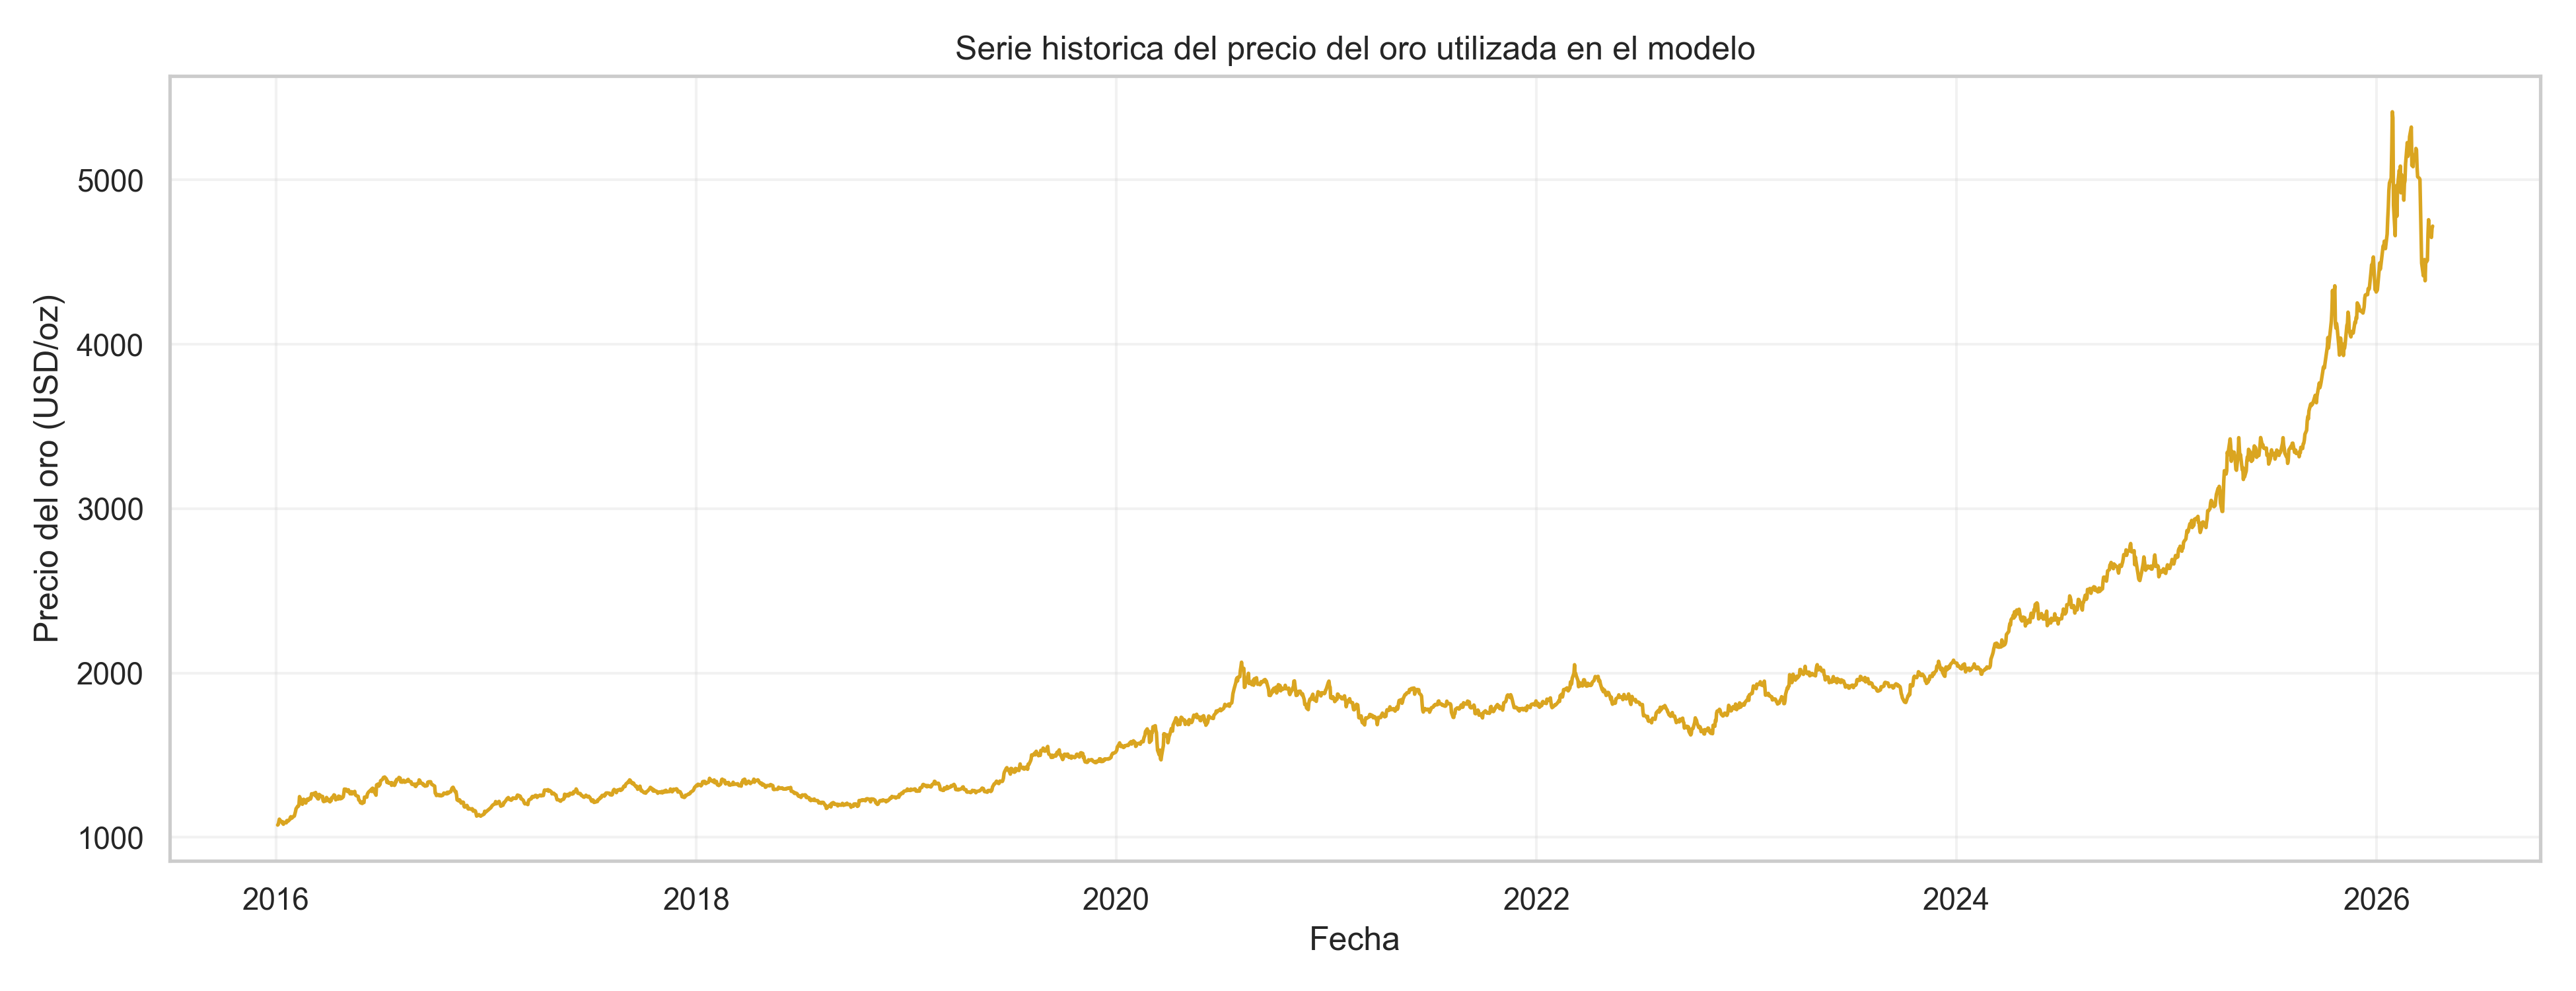
\includegraphics[width=0.95\textwidth]{01_eda_serie_oro.png}
\caption{Serie histórica del precio del oro utilizada en el modelo.}
\end{figure}

\begin{figure}[H]
\centering
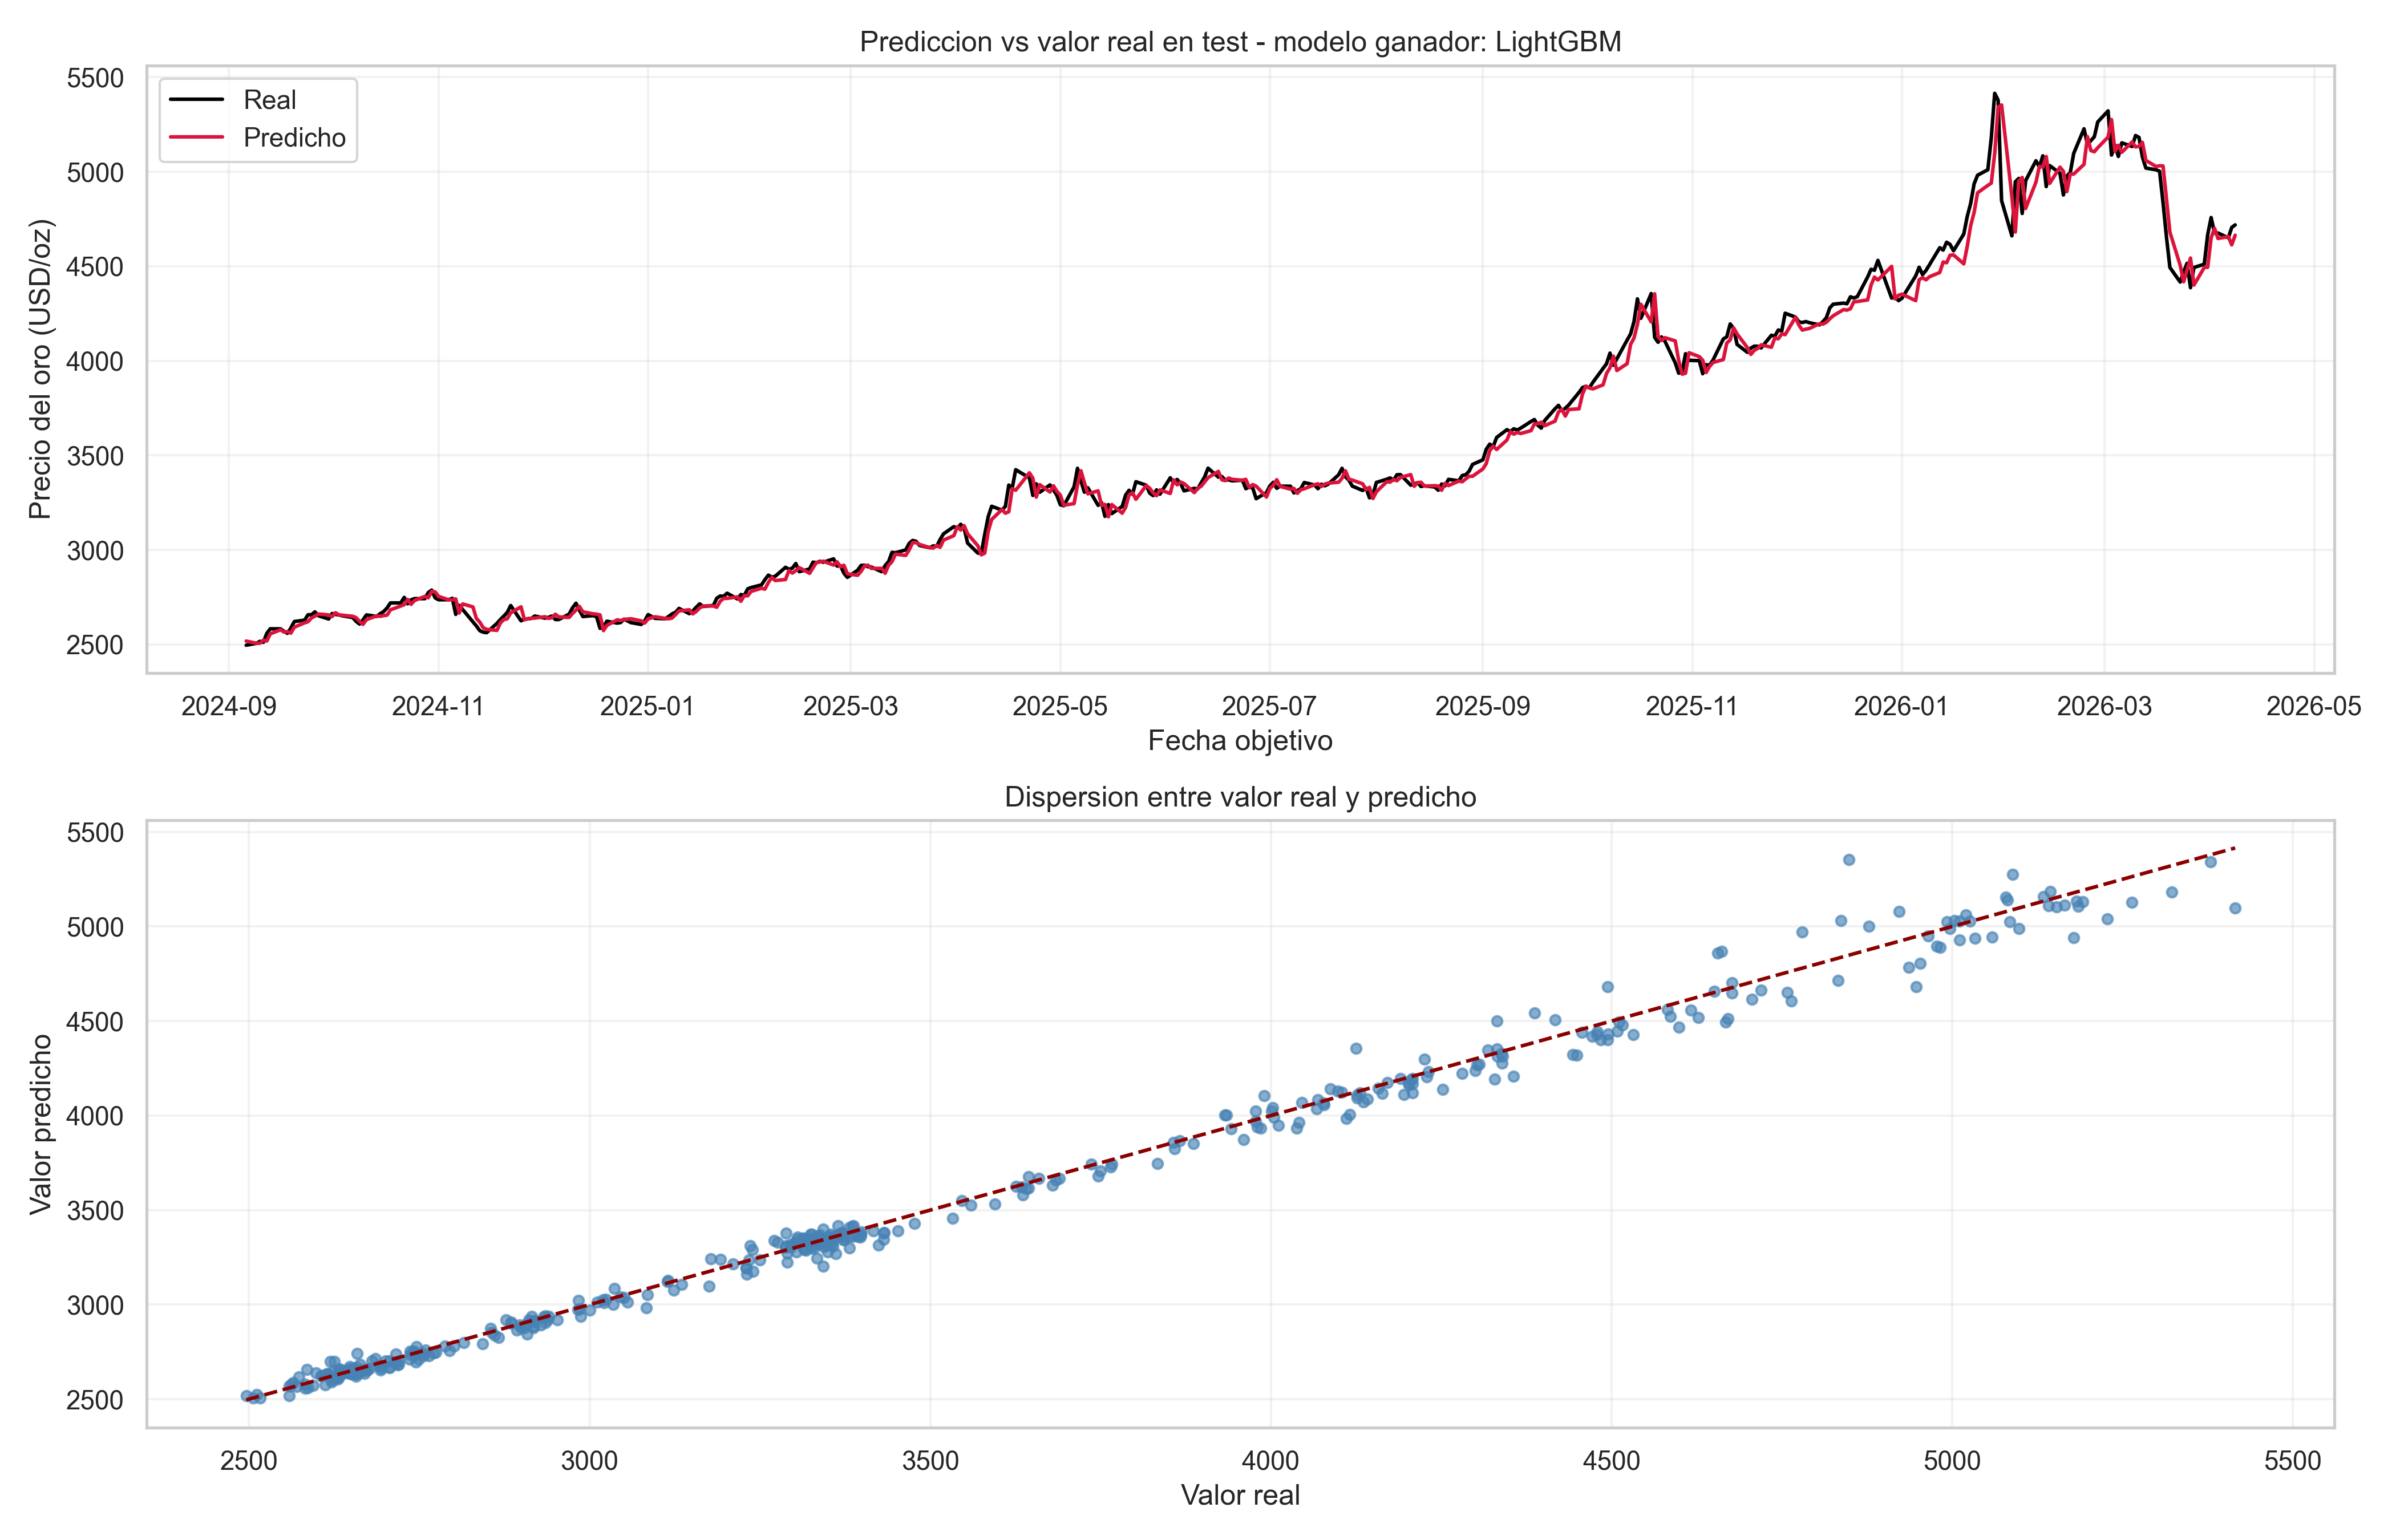
\includegraphics[width=0.95\textwidth]{02_prediccion_vs_real_test.png}
\caption{Comparación entre valores reales y predichos en test.}
\end{figure}

\begin{figure}[H]
\centering
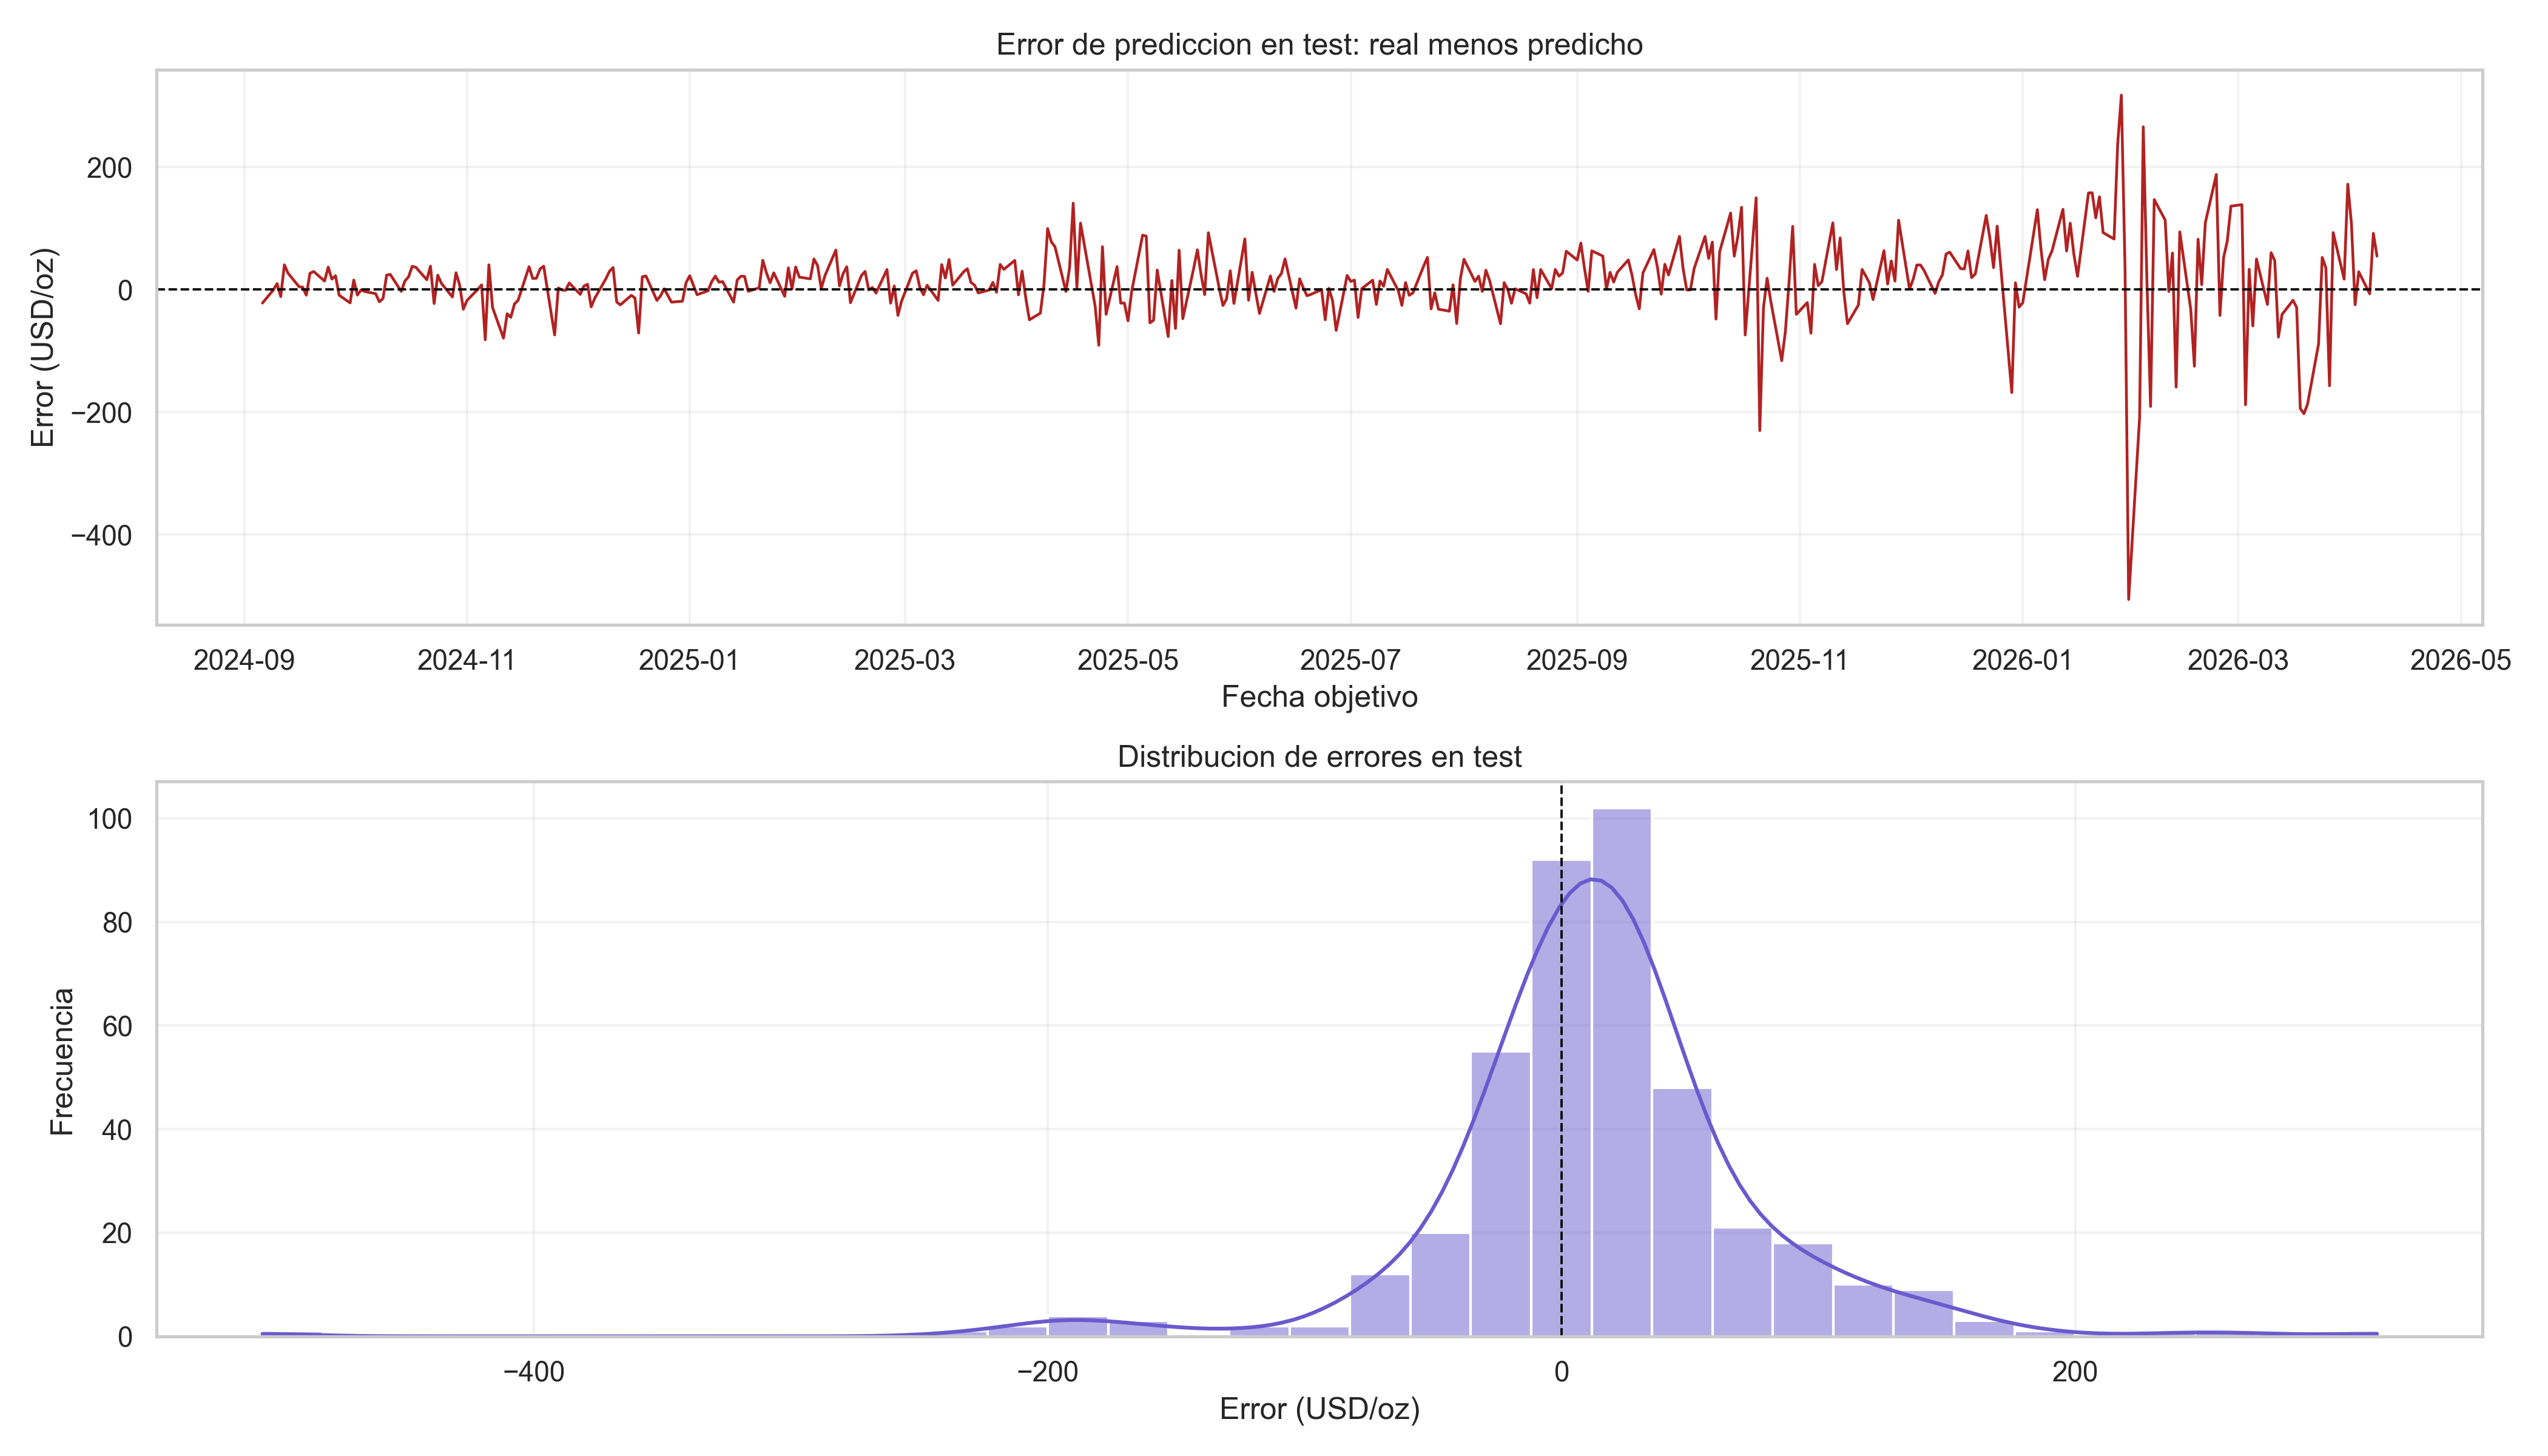
\includegraphics[width=0.95\textwidth]{03_errores_test.png}
\caption{Comportamiento y distribución de errores en test.}
\end{figure}

\begin{figure}[H]
\centering
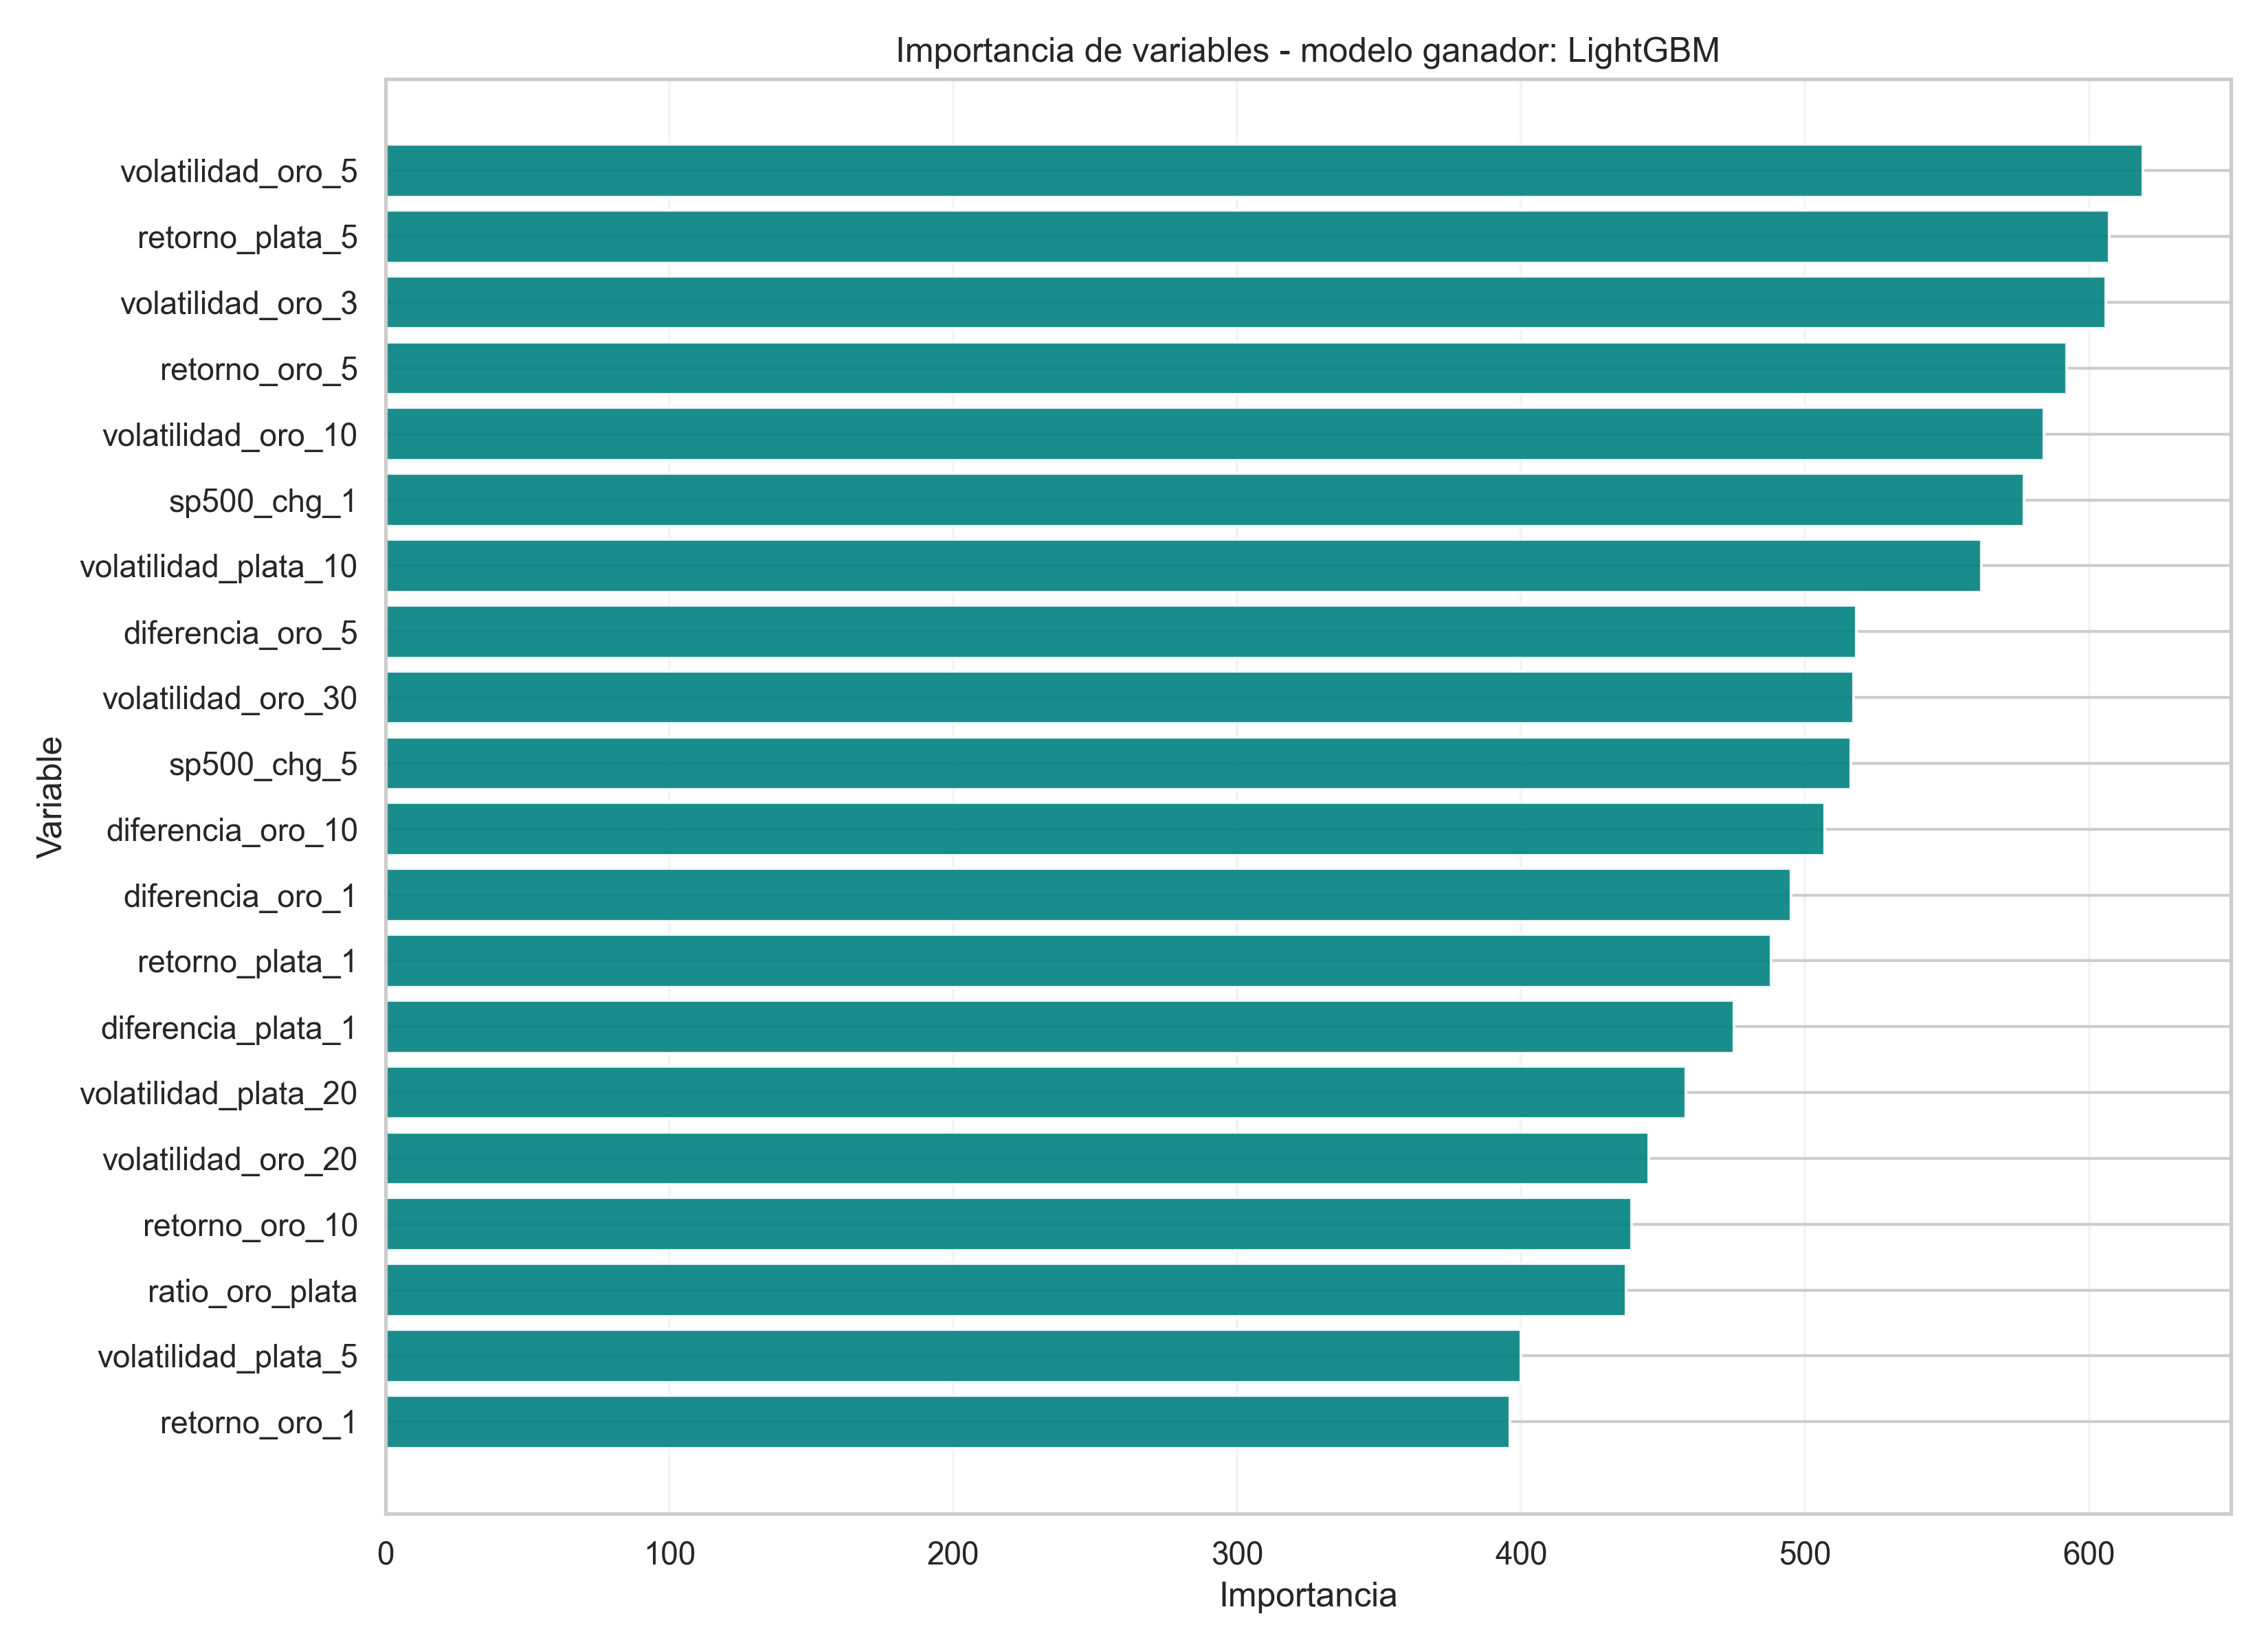
\includegraphics[width=0.95\textwidth]{04_importancia_variables.png}
\caption{Importancia de variables del modelo seleccionado.}
\end{figure}

\begin{figure}[H]
\centering
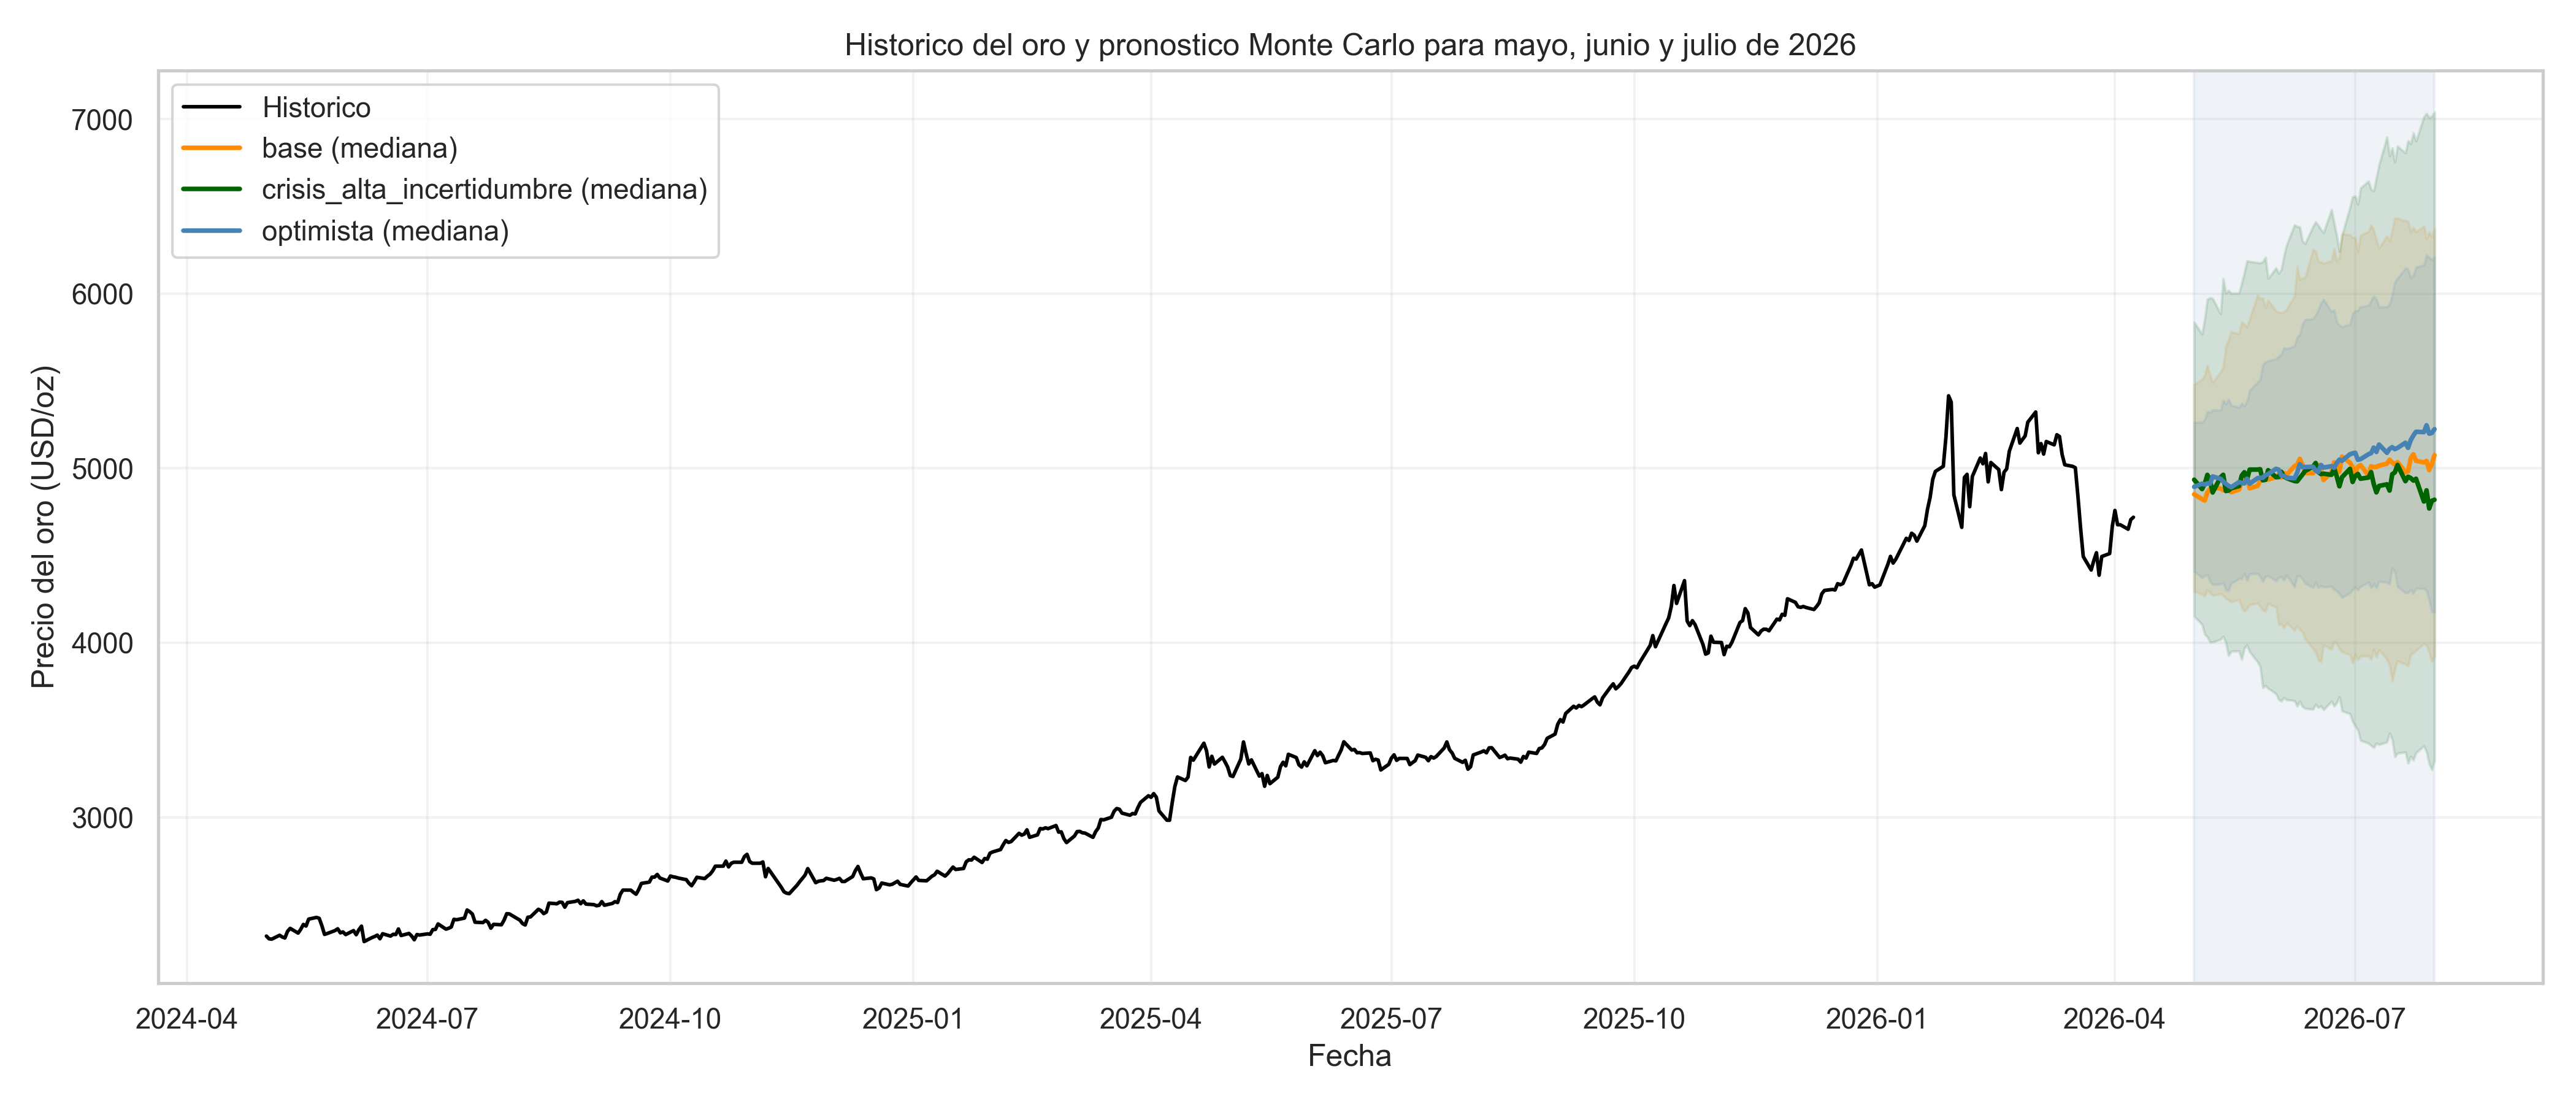
\includegraphics[width=0.95\textwidth]{06_pronostico_mayo_junio_julio_2026.png}
\caption{Pronóstico por escenarios para mayo, junio y julio de 2026.}
\end{figure}

\begin{figure}[H]
\centering
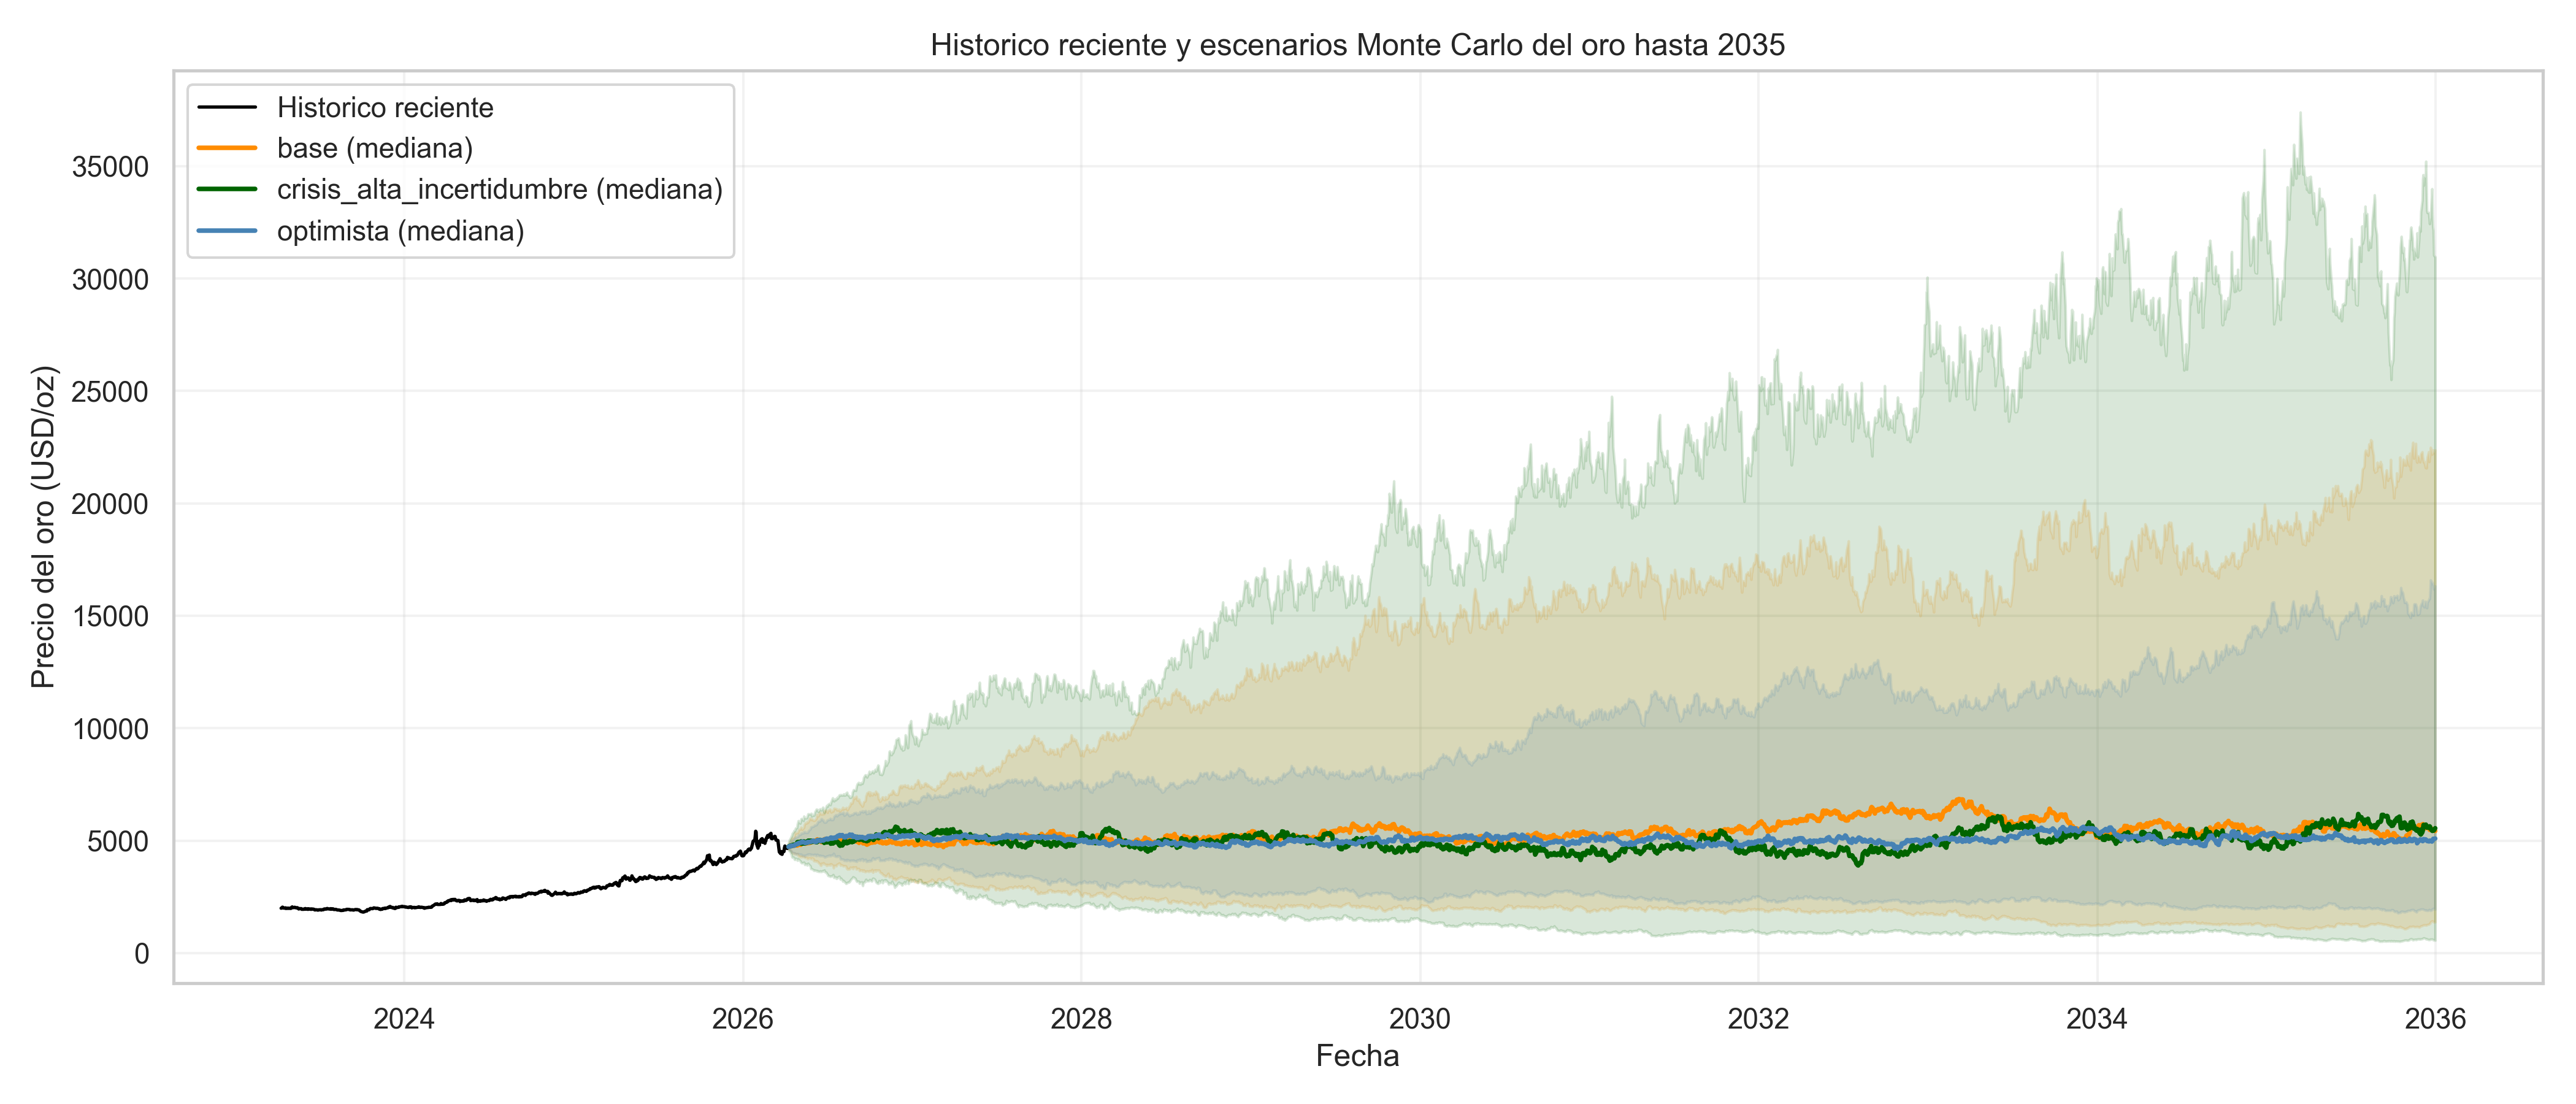
\includegraphics[width=0.95\textwidth]{07_pronostico_hasta_2035.png}
\caption{Escenarios Monte Carlo hasta diciembre de 2035. En cada escenario, la línea representa $P50$ y la banda sombreada corresponde al intervalo $P10$--$P90$.}
\end{figure}

\begin{figure}[H]
\centering
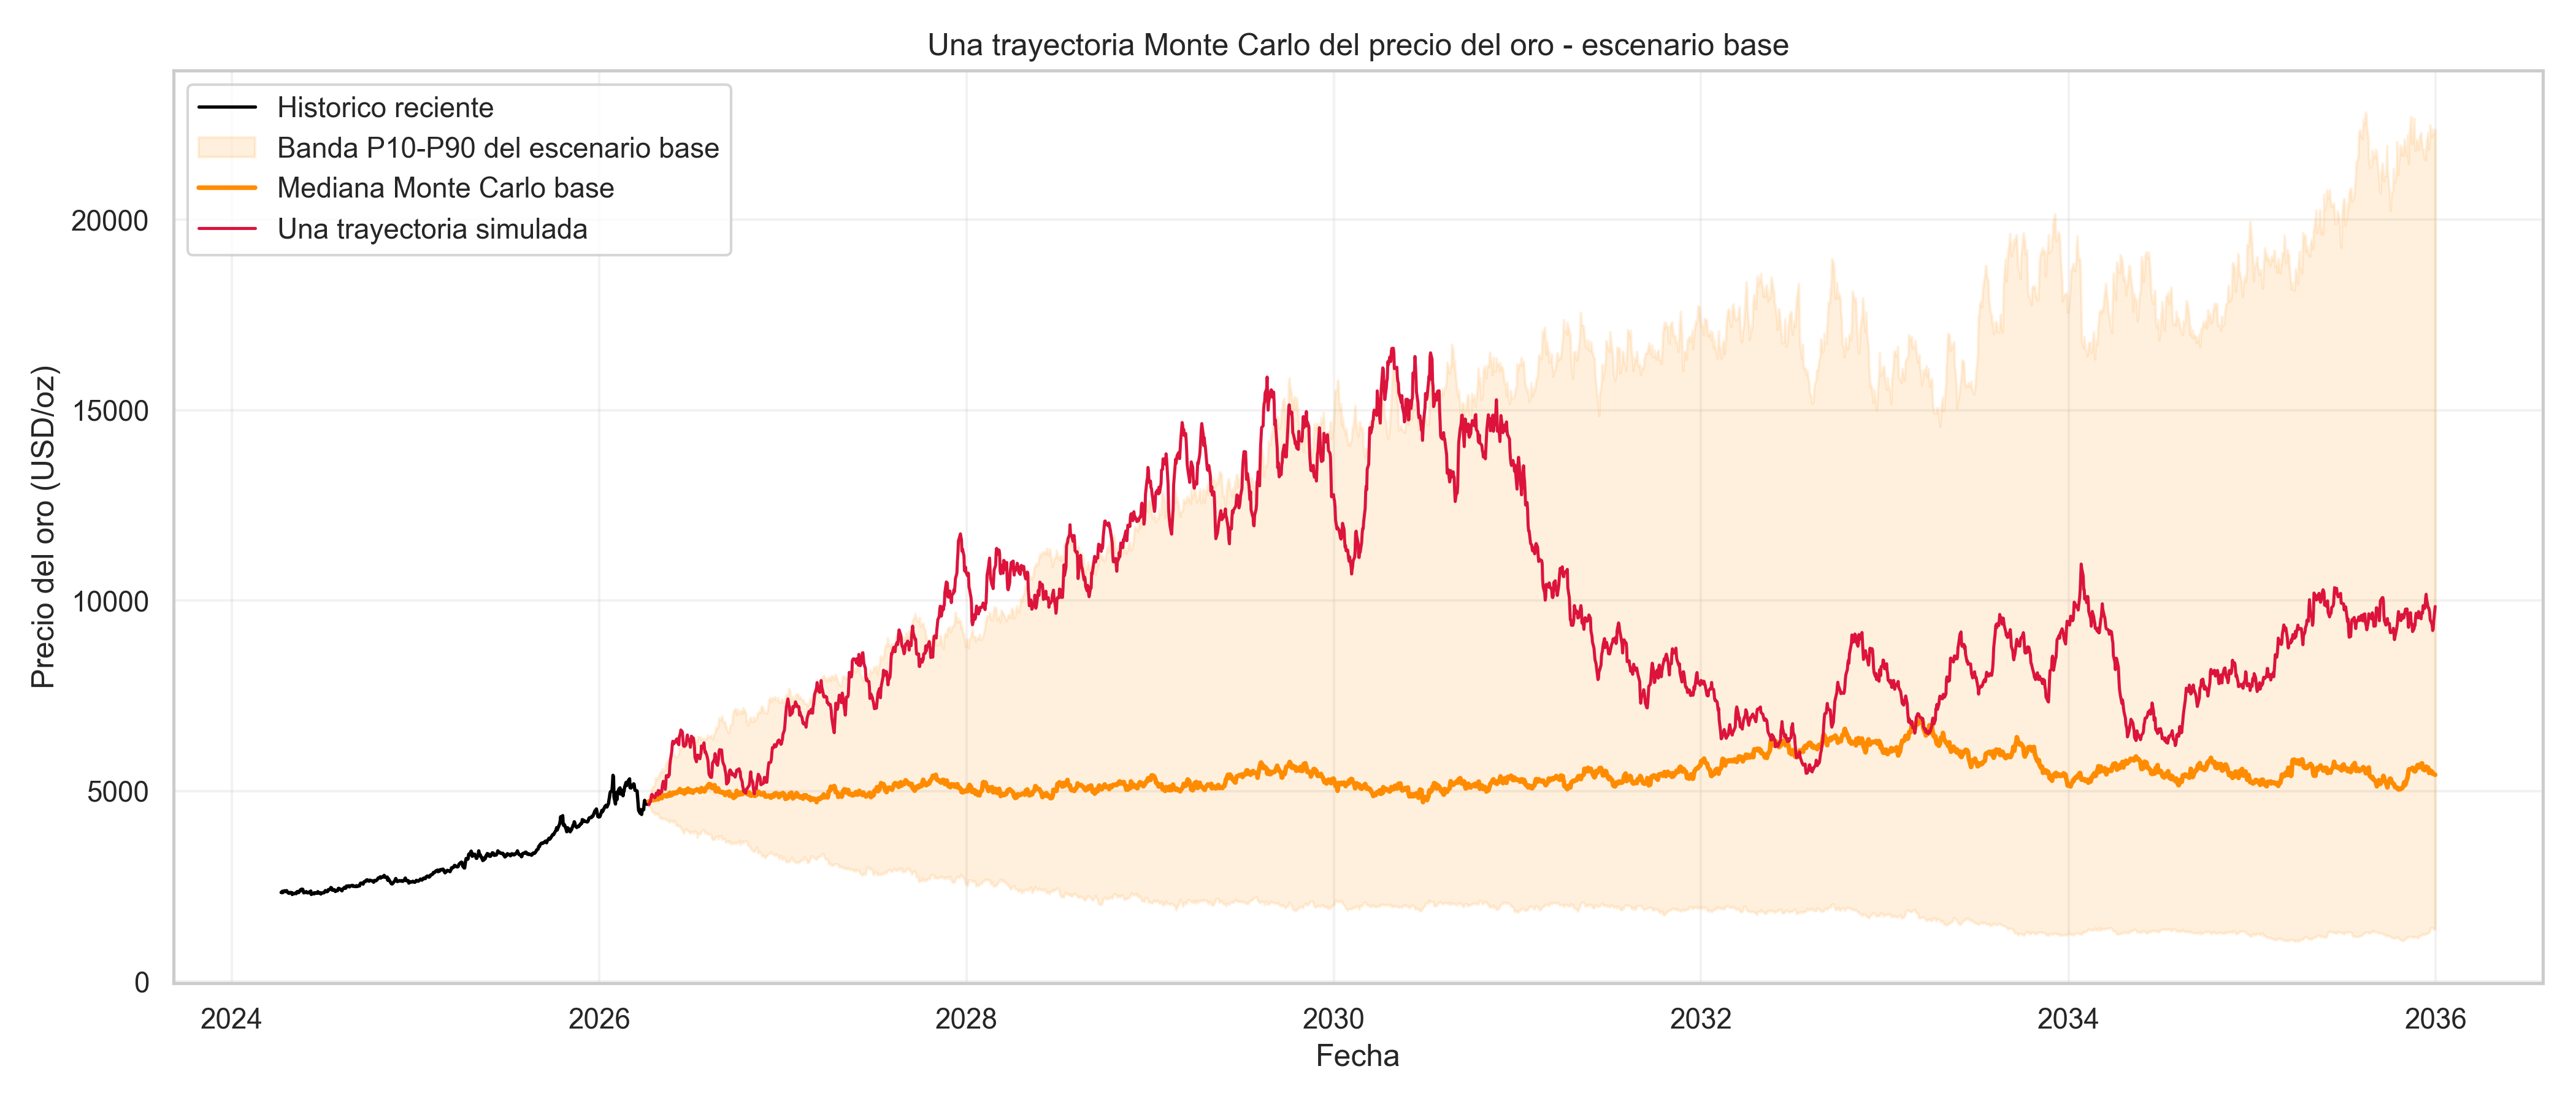
\includegraphics[width=0.95\textwidth]{09_trayectoria_unica_monte_carlo_base.png}
\caption{Ejemplo de una trayectoria individual Monte Carlo bajo escenario base. La línea roja es una ruta simulada específica; la línea naranja es el percentil $P50$ y la zona sombreada marca la banda $P10$--$P90$.}
\end{figure}

\section{Discusión}
El uso de log-retornos permitió estabilizar la variable objetivo y reducir el riesgo de fuga de información. La comparación temporal mostró que los modelos de boosting son adecuados para capturar relaciones no lineales entre variables técnicas, plata, precios NI y variables macroeconómicas. La versión inicial había seleccionado XGBoost por menor error; la versión mejorada, al incluir LightGBM, CatBoost y Optuna, encontró una configuración LightGBM con menor RMSE promedio de validación temporal.

Debe interpretarse con cautela el pronóstico de largo plazo. El horizonte hasta 2035 no representa una predicción determinista exacta, sino una simulación condicional a supuestos de escenario y a la volatilidad histórica/residual estimada. Además, algunas series externas de FRED no estuvieron disponibles en la ejecución final por errores HTTP, por lo que el modelo usó las variables efectivamente descargadas y disponibles.

\subsection{Interpretación económica}
Las variables más importantes se relacionan con volatilidad reciente del oro, retornos de la plata y variaciones del S\&P 500. Esto sugiere que el modelo capturó tres dimensiones relevantes: dinámica propia del oro, relación con otro metal precioso y condiciones financieras generales. La importancia de la volatilidad indica que los cambios bruscos recientes condicionan fuertemente el retorno esperado del siguiente día.

\subsection{Limitaciones}
El modelo depende de la calidad y disponibilidad de los datos. Algunas variables macroeconómicas externas no pudieron descargarse en la ejecución final por errores HTTP. Además, el horizonte largo acumula incertidumbre porque cada precio futuro depende del precio simulado anterior. Por tanto, los resultados a 2035 deben verse como escenarios de sensibilidad, no como predicciones puntuales garantizadas.

\subsection{Tablero de visualización}
Además del informe en PDF, se construyó un tablero HTML interactivo. Este tablero permite revisar métricas del modelo, comparación entre algoritmos, predicciones de test, importancia de variables, pronósticos de corto plazo, escenarios hasta 2035 y una trayectoria individual Monte Carlo. Su objetivo es facilitar la exploración visual de los resultados sin depender únicamente de tablas estáticas.

\section{Conclusiones}
Se construyó un flujo reproducible de machine learning para el precio del oro. El modelo inicial XGBoost fue mejorado con una comparación más amplia de algoritmos y optimización de hiperparámetros. El modelo seleccionado por validación temporal fue LightGBM optimizado con Optuna, con MAPE de 1.1323\% en test. La simulación Monte Carlo permitió generar bandas de incertidumbre y escenarios hasta 2035, útiles para análisis económico y sensibilidad en proyectos mineros. La entrega final incluye código, resultados en Excel y CSV, gráficas, documentos en LaTeX, PDFs explicativos y un dashboard interactivo.

\begin{thebibliography}{9}
\bibitem{chen2016xgboost} Chen, T. y Guestrin, C. (2016). XGBoost: A scalable tree boosting system. \textit{Proceedings of KDD}.
\bibitem{ke2017lightgbm} Ke, G. et al. (2017). LightGBM: A highly efficient gradient boosting decision tree. \textit{NeurIPS}.
\bibitem{prokhorenkova2018catboost} Prokhorenkova, L. et al. (2018). CatBoost: unbiased boosting with categorical features. \textit{NeurIPS}.
\bibitem{hyndman2021forecasting} Hyndman, R. y Athanasopoulos, G. (2021). \textit{Forecasting: Principles and Practice}.
\bibitem{cim2014ni43101} Canadian Securities Administrators. (2014). National Instrument 43-101 Standards of Disclosure for Mineral Projects.
\end{thebibliography}

\end{document}
